\newpage
\thispagestyle{plain}
\renewcommand{\sectioncolor}{chap4sub}
\section{Struktura bazy danych}

System wykorzystuje relacyjną bazę danych \textbf{PostgreSQL} \cite{postgresql_docs} w modelu \textit{Database-per-Service}. Oznacza to, że każdy z trzech głównych mikroserwisów posiada własną, odizolowaną bazę danych, co zapobiega powstawaniu silnych powiązań (\textit{tight coupling}) na poziomie schematu danych i umożliwia niezależne skalowanie usług.

\subsection{Baza danych tożsamości (IdentityService DB)}
Baza ta odpowiada za przechowywanie danych o użytkownikach, ich rolach w systemie oraz bezpieczeństwo sesji \cite{dotnet_microsoft}. Wykorzystuje ona mechanizmy \textit{Entity Framework Identity}.

\begin{itemize}
    \item \textbf{ApplicationUsers:} Przechowuje dane profilowe, skróty haseł oraz opcjonalne powiązanie z firmą (\textit{CompanyId}).
    \item \textbf{RefreshTokens:} Tabela wspierająca mechanizm bezpiecznego odświeżania sesji. Każdy token jest unikalny i powiązany z konkretnym użytkownikiem \cite{jwt_rfc}.
    \item \textbf{AuditLogs:} Rejestruje aktywność użytkowników. Pole \textit{UserId} jest opcjonalne, co pozwala na logowanie akcji systemowych lub nieudanych prób logowania.
\end{itemize}

\begin{figure}[H]
    \centering
    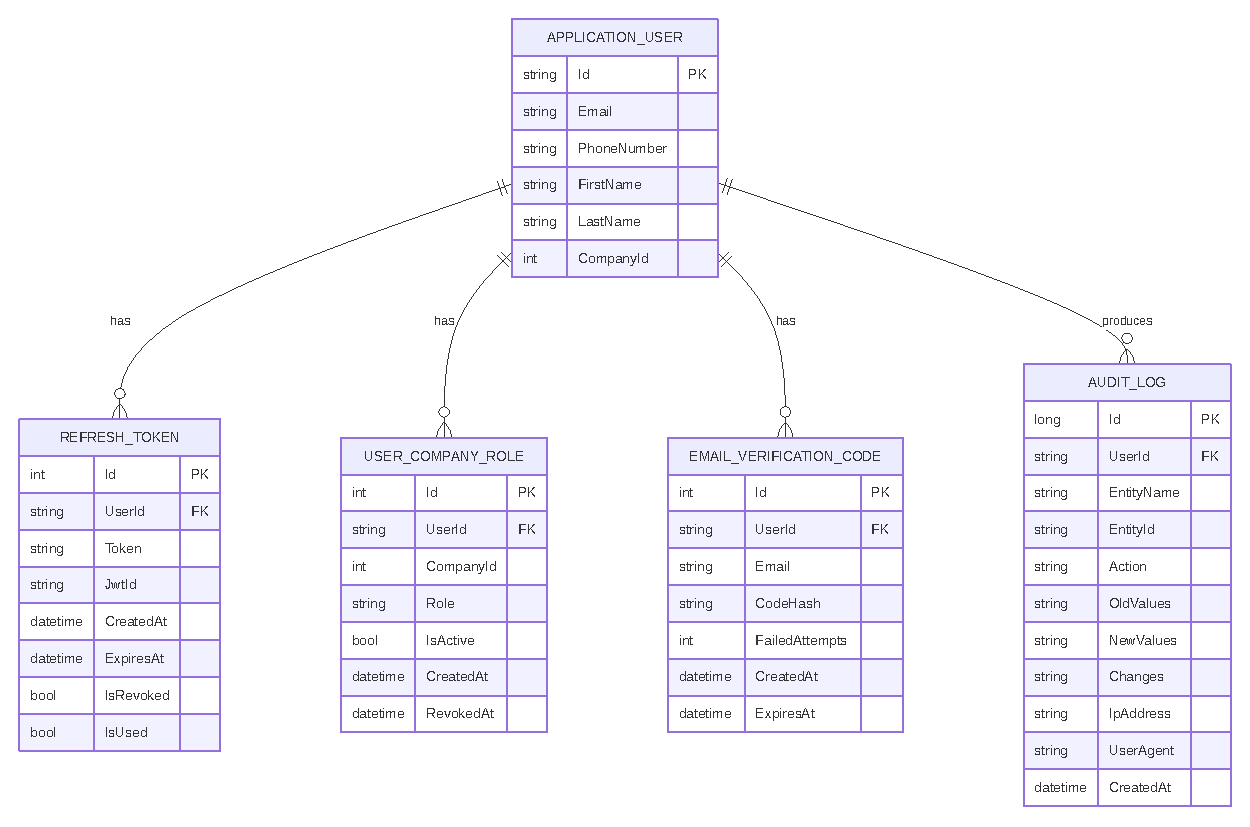
\includegraphics[width=1\textwidth]{ERD-IdentityServiceDB.pdf}
    \caption{Diagram związków encji (ERD) bazy danych mikroserwisu Identity-Service}
    \label{fig:identity_erd}
\end{figure}

\subsection{Baza danych rezerwacji (ReservationService DB)}
Na rysunku \ref{fig:reservation_erd} przedstawiono najbardziej rozbudowaną część systemu, zarządzającą logiką biznesową mikro-SaaS. Struktura wspiera model wielonajemności.

\begin{itemize}
    \item \textbf{Branches i Services:} Definiują strukturę firmy. Usługi zawierają parametry takie jak cena oraz czas trwania wraz z czasem buforowym.
    \item \textbf{Schedules i TimeSlots:} Tabele odpowiedzialne za dostępność. \textit{TimeSlot} posiada opcjonalne powiązanie z \textit{AppointmentId} – brak powiązania oznacza, że dany termin jest wolny.
    \item \textbf{Appointments:} Główna tabela rezerwacji. Implementuje mechanizm \textbf{Soft Delete}, dzięki czemu rekordy po anulowaniu nie są usuwane fizycznie, co pozwala na zachowanie spójności w tabeli \textit{BranchReviews}.
\end{itemize}

\subsection{Baza danych powiadomień (NotificationService DB)}
Baza ta została zoptymalizowana pod kątem wydajnej obsługi komunikatów i zapewnienia ich idempotentności.

\begin{itemize}
    \item \textbf{Notifications:} Przechowuje historię komunikatów \textit{In-App}, e-mail oraz SMS.
    \item \textbf{ProcessedMessages:} Kluczowa tabela dla stabilności systemu. Zawiera pole \textbf{DedupeKey}, które zapobiega ponownemu przetworzeniu tego samego zdarzenia z RabbitMQ (idempotentność konsumenta).
    \item \textbf{Templates:} Przechowuje szablony wiadomości z dynamicznymi placeholderami, które są uzupełniane danymi z pola \textit{RelatedAppointmentId}.
\end{itemize}

\begin{figure}[H]
    \centering
    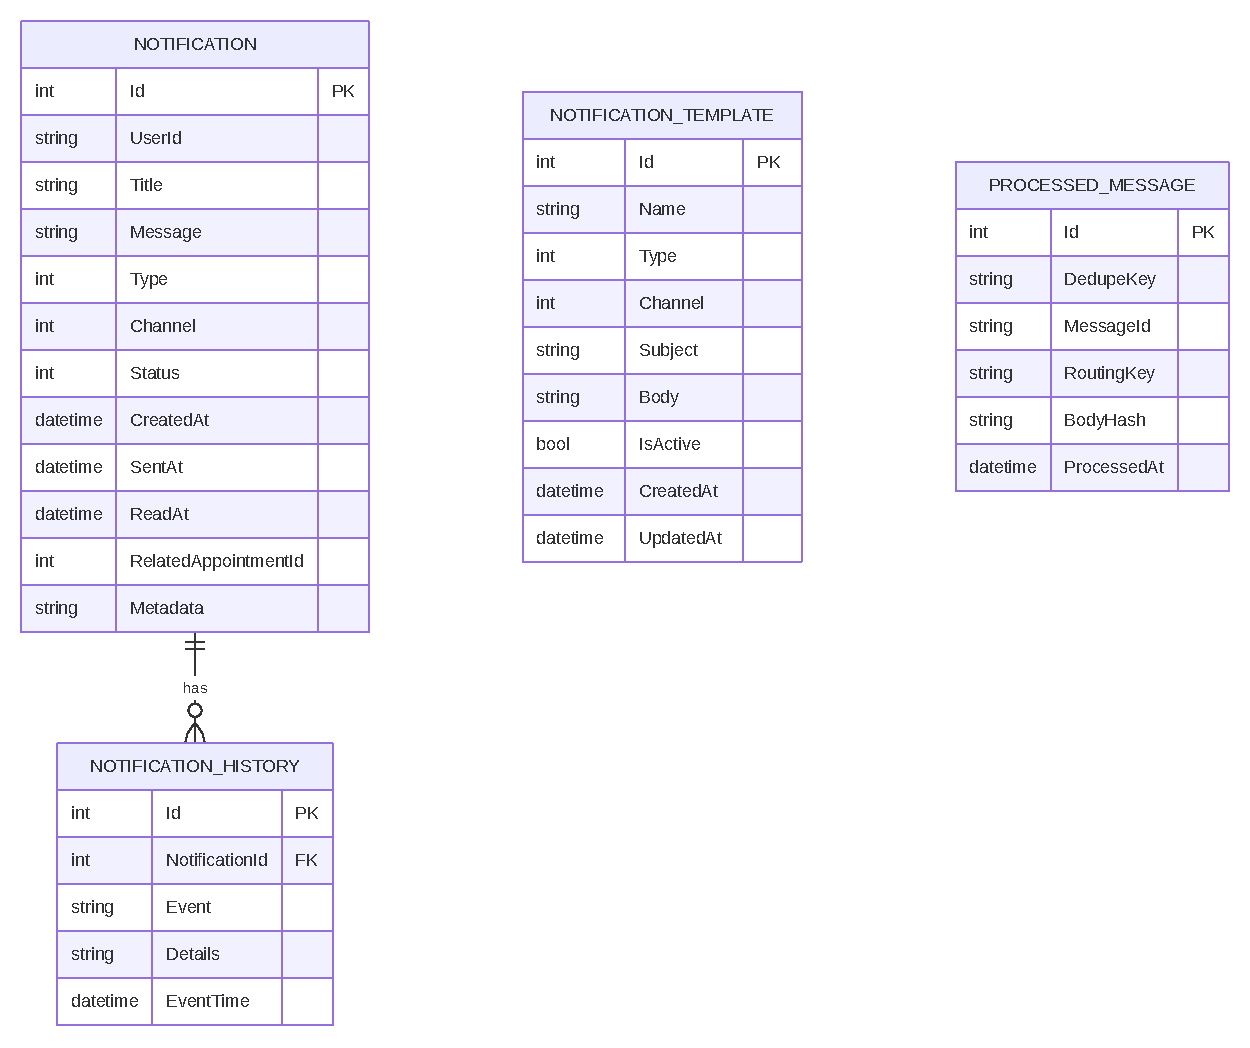
\includegraphics[width=1\textwidth]{ERD-NotificationServiceDB.pdf}
    \caption{Diagram związków encji (ERD) bazy danych mikroserwisu Notification-Service}
    \label{fig:notification_erd}
\end{figure}

\subsection{Integralność danych w architekturze rozproszonej}
Z racji fizycznej separacji baz danych, system nie wykorzystuje tradycyjnych więzów integralności (\textit{Foreign Keys}) pomiędzy serwisami. Zamiast tego zastosowano mechanizm \textbf{spójności ostatecznej} (\textit{Eventual Consistency}):
\begin{enumerate}
    \item Identyfikatory użytkowników (GUID) są przekazywane w tokenach JWT \cite{jwt_rfc} i zapisywane jako zwykłe pola typu UUID w bazie rezerwacji.
    \item Zmiany danych (np. zmiana statusu rezerwacji) są propagowane asynchronicznie przez broker komunikatów RabbitMQ \cite{rabbitmq_docs}.
    \item Mechanizm \textit{Audit Log} w każdej bazie pozwala na odtworzenie stanu systemu w przypadku niespójności.
\end{enumerate}

% Zdjecie Reservation z ograniczona wysokoscia na koncu rozdzialu
\begin{figure}[H]
    \centering
    % Ograniczenie do 20cm wysokosci przy zachowaniu proporcji
    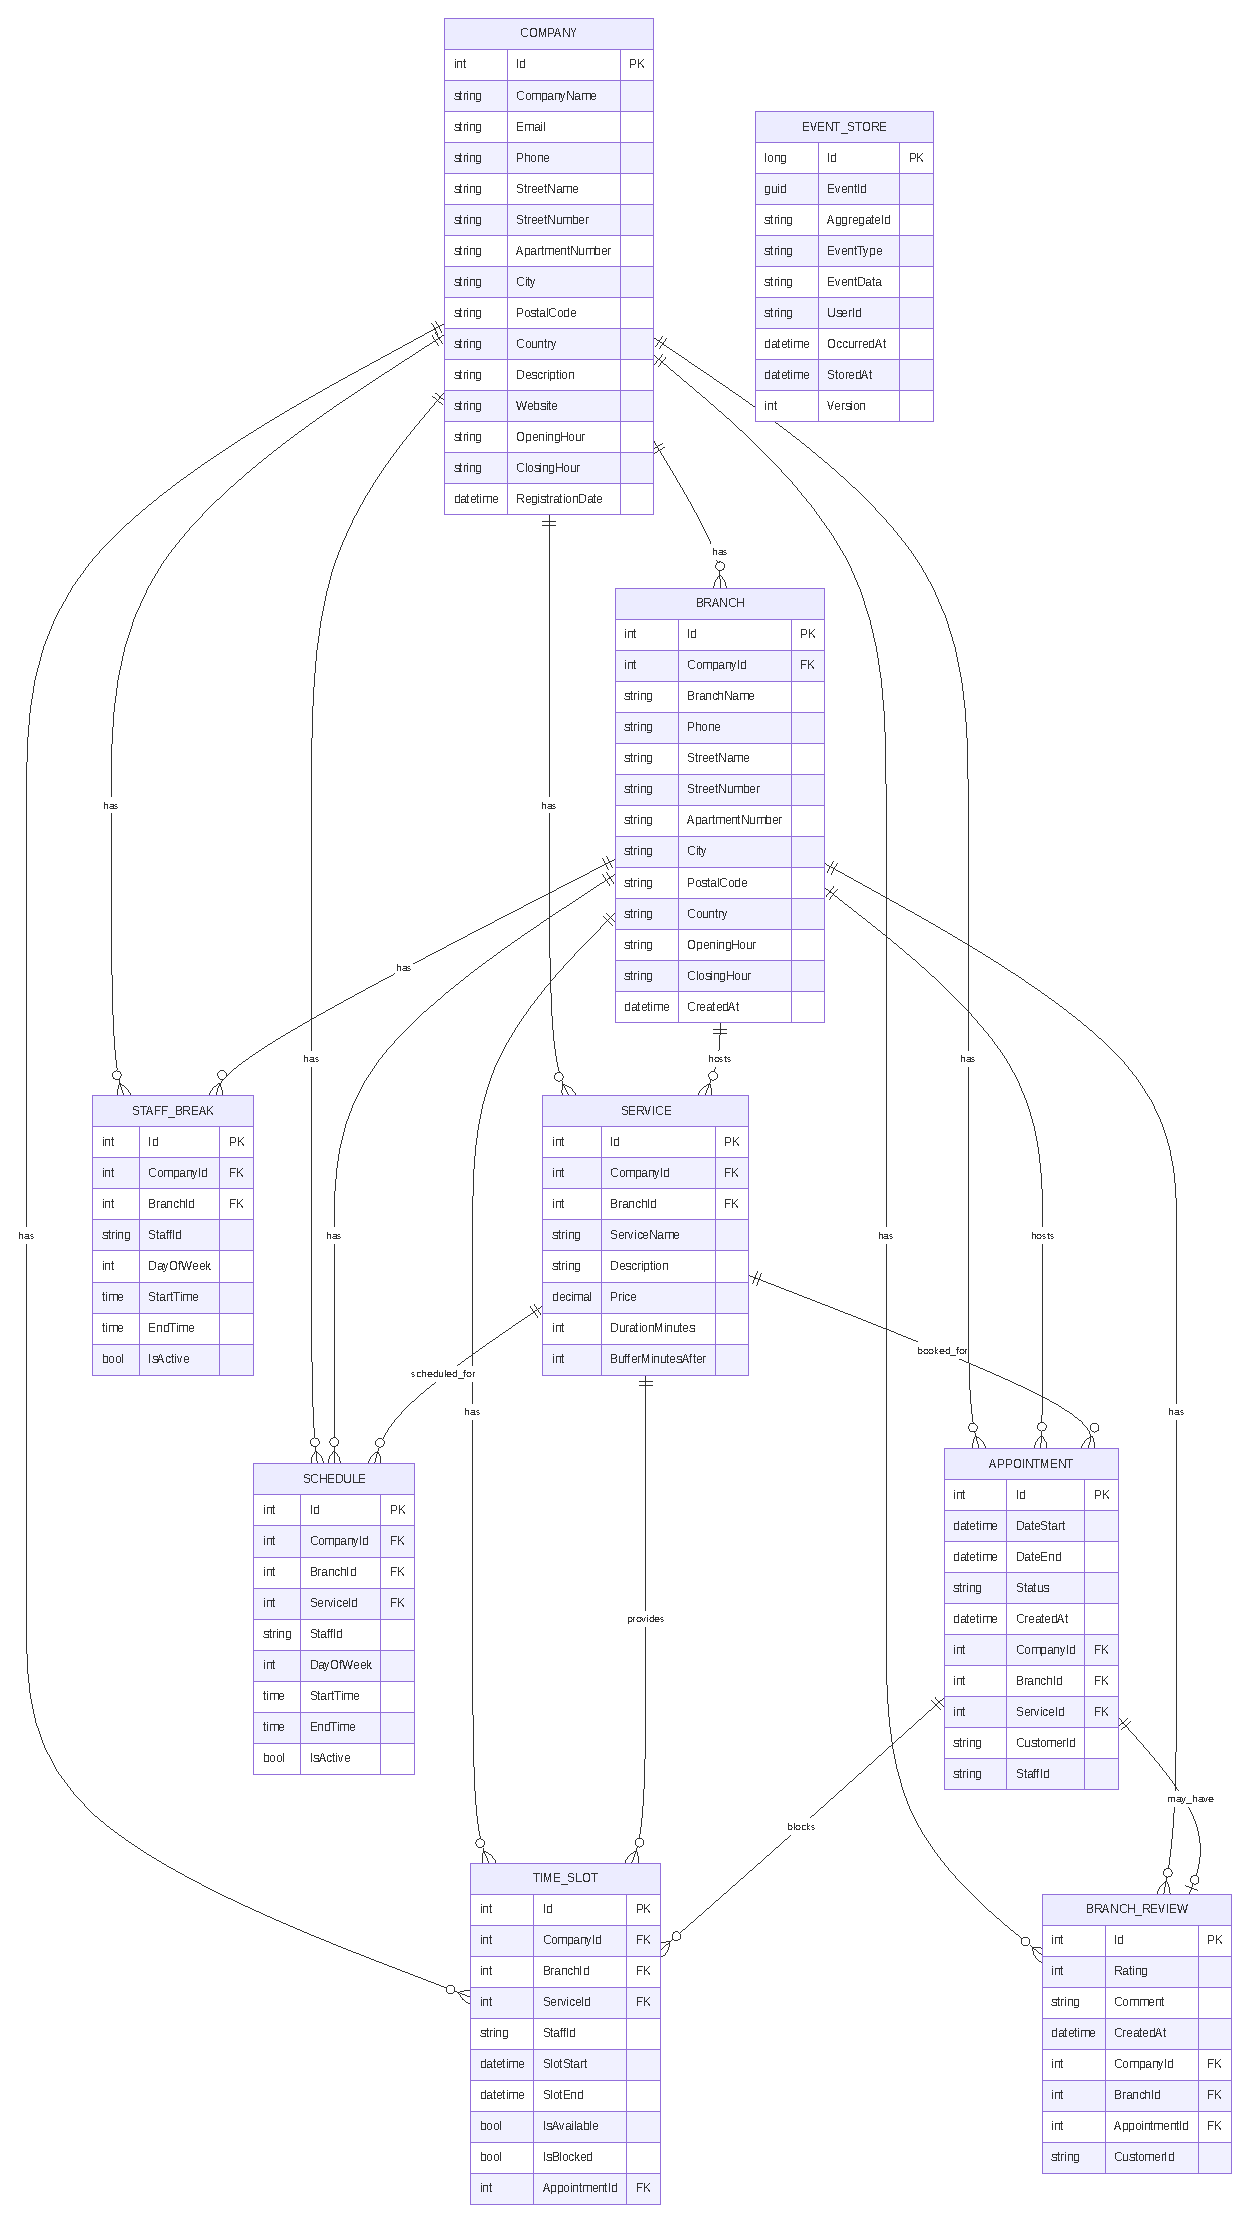
\includegraphics[height=24cm, width=1\textwidth, keepaspectratio]{ERD-ReservationServiceDB.pdf}
    \caption{Diagram związków encji (ERD) bazy danych mikroserwisu Reservation-Service}
    \label{fig:reservation_erd}
\end{figure}